\section{Funktionsweise von Vektoruhren}
\label{cap:funktionsweise}
In diesem Kapitel wird die allgemeine Funktionsweise von Vektoruhren behandelt. Mittels geeigneten Beispielen wird die Kommunikation in einem einfachen verteilten System illustriert, um die Funktionsweise von Vektoruhren innerhalb der Kommunikation zu zeigen. Zuletzt wird auf das System eingegangen, welches im Rahmen dieser Arbeit in der Programmiersprache C\# implementiert wurde.
\subsection{Prinzipielle Funktionsweise}
\label{prinzipFunktion}
Wie bereits beschrieben wurde, bilden Vektoruhren eine Erweiterung der Lamportuhr. Dabei wird in jedem Prozess im System ein Integer als Zähler in der Vektoruhr gespeichert. Im Allgemeinen werden durch eine Vektoruhr Zeitstempel mit Events im System assoziiert \cite{Baldoni:2002:FDC:1435723.1437765}[S. 3].

Jeder Prozess im System besitzt seine eigene Vektoruhr in der Form eines Vektors $VC_i[1...n]$, wobei alle Elemente der Uhr mit $0$ initialisiert werden. Im Laufe der Kommunikation werden durch die verschiedenen, verteilten Prozesse Nachrichten untereinander verschickt. Damit durch den Einsatz von Vektoruhren nachvollzogen werden kann, wie die Zeitlichen Reihenfolge solcher Events aussieht, müssen die entsprechenden Uhren jeweils bei auftreten eines Events angepasst werden.
Die Uhr eines Prozesses wird wie folgt verwaltet und aktualisiert \cite{Baldoni:2002:FDC:1435723.1437765}[S. 4]:

\begin{itemize}
	\item[R1]Jedes mal, wenn ein Prozess $P_i$ ein Event auslöst, muss dieser seine Vektoruhr für den Eintrag $VC_i$ um Eins inkrementieren, es gilt  $VC_i[i] := VC_i[i] + 1$. Dadurch verdeutlicht der Prozess, dass er ein Event verarbeitet hat und signalisiert dies den anderen Prozessen durch aktualisieren seiner Vektoruhr 
	\item[R2]Sendet ein Prozess $P_i$ eine Nachricht $m$, so hängt er seine aktuelle Vektoruhr $VC_i$ an die zu sendende Nachricht an. Auf diese Weise gelangt die Uhr zu dem Empfänger der Nachricht.
	\item[R3]Empfängt ein Prozess $P_i$ eine Nachricht, so muss er seine Vektoruhr aktualisieren. Dabei geht er wie folgt vor: $VC_i = \max(VC_i, m.VC)$. Dies bedeutet, dass der Prozess für jedes Element seiner Vektoruhr überprüft, ob der Wert in der Uhr der Nachricht größer als der eigene ist. Sollte dies der Fall sein, wird der eigene Wert an dieser Stelle mit dem Wert aus der anderen Uhr überschrieben.\label{R3}
\end{itemize}

Die Werte innerhalb einer Vektoruhr $VC_i$ haben eine besondere Bedeutung für den Prozess $P_i$. $VC_i[i]$ gibt die Anzahl an Events an, welche $P_i$ zu dem Zeitpunkt des Betrachtens verarbeitet hat. Die anderen Werte der Uhr ($VC_i[j]$ mit $j \neq i$) zeigen an, dass sich alle Events welche durch den Prozess $P_j$ verarbeitet wurden kausal betrachtet in der Vergangenheit von $P_i$ befinden. Sie geben sozusagen an, was der Prozess $P_i$ über die Zeiten der anderen Prozesse weiß, diese Information kann sich zu dem Zeitpunkt jedoch bereits von den tatsächlichen Zeiten in den anderen Prozessen unterscheiden. Da jeder Prozess lediglich seinen Zähler in der Vektoruhr erhöhen darf, hat dieser zu jedem Zeitpunkt den aktuellsten Stand seiner lokalen Zeit. \cite{singhal1992efficient}[S. 48]

Eine Besonderheit der Vektoruhren besteht im Vergleich von Uhren untereinander. Dies wird notwendig, sobald ein Prozess eine Nachricht erhält und diese verarbeiten muss. Verarbeiten bedeutet im Kontext von Vektoruhren, dass die empfangene Nachricht an eine Anwendungsschicht weitergegeben wird. Warum dies notwendig ist, wird in Abschnitt~\ref{RolleDerAnwendung} genauer erläutert.

Wie in Bedingung R3 unter \textit{\ref{R3}~-~\nameref{R3}} zu sehen, muss der Prozess seine Uhr entsprechen der mitgeschickten Vektoruhr der Nachricht aktualisieren. Der Vergleich zwischen der eigenen und der empfangenen Uhr muss dann bei Bedarf auf Anwendungsebene geschehen, denn dort wird entschieden, was mit der angekommenen Nachricht geschieht.

Für zwei zu vergleichende Uhren $VC_1$ und $VC_2$ gibt es folgenden Beziehungen:

\begin{eqnarray}
&VC_1 \leq VC_2& \text{ genau dann, wenn } \forall i : VC_1[i] \leq VC_2[i] \\
	&VC_1 < VC_2& \text{ genau dann, wenn } VC_1 \leq VC_2 \wedge VC_1 \neq VC_2 \\
	&VC_1 \mid \mid VC_2& \text{ genau dann, wenn } \neg(VC_1 < VC_2) \wedge \neg(VC_2 < VC_1)
\end{eqnarray}
\cite{mattern1989virtual}[S. 127, Definition 4]

Fall~(1) bedeutet, dass eine Uhr $VC_1$ kleiner oder gleich $VC_2$ ist, wenn jedes Element von $VC_1$ kleiner oder gleich dem entsprechenden Element in $VC_2$ ist. Der zweite Fall~(2) liegt vor, wenn Fall~(1) zutrifft und zusätzlich kein Element in $VC_1$ gleich dem entsprechenden Element in $VC_2$ ist. 
Der letzte Fall~(3) ist ein Besonderer Fall. Dieser trifft ein wenn nicht entschieden werden kann, welche Uhr neuer oder älter beziehungsweise nach der obigen Definition größer oder kleiner ist als die andere. Die entsprechenden Nachrichten wurden sozusagen gleichzeitig abgeschickt. Dieser im Englischen als \qq{Concurrent} bezeichnete Fall stellt ein großes Problem für Systeme dar, die Vektoruhren für die zeitliche Synchronisation der Kommunikation nutzen. Auf diesen Sonderfall wird im nächsten Kapitel genauer eingegangen.

\subsection{Beispiel einer Kommunikation}

Um die Funktionsweise von Vektoruhren genauer zu beschreiben, wird nun zunächst anhand zweier einfacher Beispiele die Kommunikation in einem System mit drei Prozessen sowie die Verarbeitung der Vektoruhren eines jeden Prozesses gezeigt. Das erste Beispiel behandelt eine Kommunikation, die konfliktfrei abläuft und in der die drei Prozesse des verteilten Systems einzelne Nachrichten an beliebige anderen Prozesse senden. In dem zweiten Beispiel wird eine konfliktbehaftete Kommunikation illustriert, bei der durch abgesendete und ungeordnete Broadcasts Statusaktualisierungen mitgeteilt werden.

\subsubsection{Konfliktfreie Kommunikation}
Am Anfang weiß jeder Prozess nur seine lokale Zeit, der Wert $VC_i$ für Prozess $P_i$ wird deshalb auf $0$ gesetzt. Da der Prozess noch keine Kenntnis über die anderen Teilnehmer im System hat, werden die anderen Einträge mit \qq{$-$} initialisiert.

Zu Beginn sendet in dem in Abbildung~\ref{figure:kommBeispiel1} abgebildeten Beispiel Prozess $P_3$ eine Nachricht an $P_1$. Er erzeugt dabei ein Event und muss deshalb zunächst seine lokale Vektoruhr inkrementieren, der Wert $VC_3[3]$ wird also um $1$ erhöht. Die Uhr hat nun den Wert \vc{-}{-}{1}. Anschließend wird die lokale Uhr an die zu sendende Nachricht angehängt und diese verschickt.
Nun empfängt Prozess $P_1$ diese Nachricht. Gemäß Regel R1 muss zunächst die lokale Uhr entsprechend der mitgeschickten Uhr aktualisiert werden. Da in jedem Feld der Uhr das Maximum genommen wird, wird die lokale Uhr von $P_1$ nach der Aktualisierung von \vc{0}{-}{-} auf \vc{1}{-}{1} geändert. Da das Empfangen einer Nachricht auch als Event angesehen wird, erhöht sich auch der Wert für den lokalen Zähler von $P_1$ innerhalb der Uhr um $1$.

\begin{figure}[ht]
	\centering
	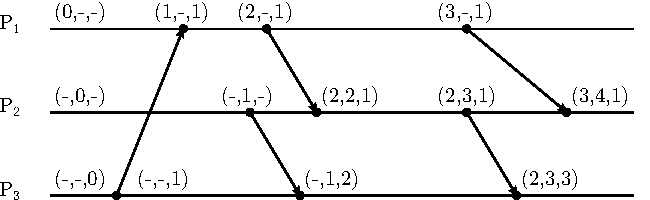
\includegraphics[width=10cm]{KommBeispiel1.pdf}
	\caption[Beispiel einer konfliktfreien Kommunikation]{Ablauf der Kommunikation dreier Prozesse mit Veranschaulichung der dabei auftretenden Vektoruhren.}
	Quelle: Nachgezeichnet aus \cite{Baldoni:2002:FDC:1435723.1437765}[S. 5]
	\label{figure:kommBeispiel1}
\end{figure}
\FloatBarrier

In diesem Beispiel kommen alle Nachrichten passend nacheinander an und es kann zu keinen Konflikten in der Ausführungsreihenfolge kommen. Das Nachfolgende Beispiel verdeutlicht den Fall, dass gesendete Nachrichten auch von anderen Nachrichten abhängig und während der Übertragung verzögert ankommen können, was ein Problem eines einfachen Systems mit Vektoruhren darstellt.

\subsubsection{Kommunikation mit Konflikten}

Das im Folgenden beschriebene Beispiel lässt sich auf ein verteiltes System anwenden, welches ein Bankensystem mit einem Konto und drei unabhängigen Bankautomaten als Prozesse abbildet. Jeder Automat speichert als Information den aktuellen Kontostand ab. Diese Architektur dient hier lediglich als Vereinfachung und entspricht nicht einem realen Bankensystem, welches mit einer Client-Server-Architektur arbeiten würde. 

Wird eine Aktion beziehungsweise ein Event ausgeführt, zum Beispiel eine Ein- oder Auszahlung, so sendet der Automat per Broadcast eine Nachricht mit der Aktualisierung und seiner Vektoruhr an alle anderen Automaten im System.

\begin{figure}[ht]
	\centering
	\includegraphics[width=10cm]{KommBeispiel2.pdf}
	\caption[Beispiel einer konfliktbehafteten Kommunikation]{Ablauf der Kommunikation in einem Bankensystem, bei dem durch einen Broadcast ein Konflikt beim Vergleich von Vektoruhren auftritt.}
	\label{figure:kommBeispiel2}
\end{figure}
\FloatBarrier

Zu Beginn werden die Vektoruhren der Prozesse wie im vorherigen Beispiel beschrieben initialisiert. Das erste Event wird an Prozess 2 ausgelöst. Hier passiert beispielhaft eine Ein- oder Auszahlung, die tatsächliche Aktion spielt für das Beispiel weniger eine Rolle als die Tatsache, dass sich der Kontostand geändert hat. Durch die Änderung des Kontostandes wird also im System ein Event ausgelöst. Der Prozess $P_2$ schickt nun einen Broadcast mit dem aktualisierten Kontostand und seiner lokalen, ebenfalls aktualisierten Uhr an die übrigen Bankautomaten. Diese empfangen die Nachricht und behandeln sie entsprechend.

Der Konflikt passiert in diesem Beispiel bei den nächsten beiden Events. Zunächst wird an Prozess $P_3$ ein Event ausgelöst. Dieser versucht nun, einen Broadcast an die anderen Automaten zu senden, was jedoch aus technischen Gründen fehlschlägt, so dass die Aktualisierungsnachricht nicht bei den übrigen Prozessen ankommt. Zeitgleich zu diesem Event wird auf Automat $P_1$ der Kontostand aktualisiert. Der Zeitpunkt \qq{Zeitgleich} bedeutet hier jedoch nicht zwangsweise, dass die Events tatsächlich zu der gleichen, physikalischen Zeit passiert sind, sondern lediglich im Sinne der Reihenfolge von auftretenden Events. Der Prozess sendet nach der Aktualisierung des Kontos sowie seiner lokalen Uhr den Broadcast. Der eigentliche Konflikt entsteht nun an Prozess $P_3$, denn dessen Änderung am Konto ist nicht in das Event von $P_1$ mit eingeflossen, die beiden Aktionen wurden also parallel ausgeführt und es kann durch einen Vergleich der Vektoruhren nicht entschieden werden, welches Event vor dem anderen stattgefunden hat. Nach den Regeln für den Vergleich von Vektoruhren in Abschnitt~\ref{prinzipFunktion} entspricht dies dem dritten Fall.

Eine Praktische Bedeutung hätte dies, wenn in $P_3$ bei einem Kontostand von 100 \euro{} der Betrag 60 \euro{} abgehoben würde. Werden nun zeitgleich an Automat $P_1$ 80 \euro{} abghoben, so hat der Automat $P_3$ nun seinen lokalen Kontostand über 20 \euro{} sowie den empfangenen von 40 \euro{}. Ein solcher Konflikt kann und darf nicht auf der Ebenen der Vektoruhren gelöst werden. Er muss an eine Anwendungs-API weitergereicht werden, was im Abschnitt~\ref{RolleDerAnwendung} genauer erläutert wird.  

\subsection{Umsetzung in C\#}
\label{vectorClockImpl}
Wie bereits erwähnt stellt das im Rahmen dieser Arbeit entwickelte System ein Bankensystem dar. Um den Aufwand der Implementierung etwas zu reduzieren, wurde eine Peer-to-Peer Architektur entwickelt, bei der die drei Prozesse des Systems die Daten direkt halten und nicht wie beispielsweise bei einer Client-Server-Architektur auf ein Backend zugreifen. Das System stellt sozusagen eine verteilte Datenbank dar.
Des weiteren besteht in dem System lediglich eine \textit{Eventual Consistency}, wie sie bereits in Abschnitt~\ref{lbl:consistency} eingeführt wurde. Der konsistente Zustand besteht demnach erst nach einer gewissen Zeitspanne. Problematisch wird es, sobald in dem Bankenszenario Zinsen für gewisse Geldbeträge ausgerechnet werden sollen. In diesem Fall reich eine eventual consistency nicht aus und man müsste auf eine totale Ordnung mit Lamport-Uhren zurückgreifen \cite{Tanenbaum2007}[S. 248].

Für die Umsetzung dieses Themas wurde C\# als Programmiersprache ausgewählt. Damit die zeitliche Synchronisation mittels Vektoruhren möglichst realitätsnah simuliert werden kann, wurden drei virtuelle Maschinen mit dem Betriebssystem Windows 8.1 aufgesetzt. Diese befinden sich im Hochschulnetzwerk und können per Remote Desktop bedient werden. Um die effizienz der Entwicklung zu erhöhen, wurde die Addressierung der Nodes durch IPEndPoints umgesetzt. Dies stellt einen generellen Endpunkt des IP-Protokolls bestehend aus IP-Addresse und einem Port dar. Dadurch konnte das gesamte System zu Testzwecken auch auf nur einem, lokalen Computer ausgeführt und getestet werden.

\subsubsection{Genereller Aufbau des Programms}

\begin{figure}[ht]
	\centering
	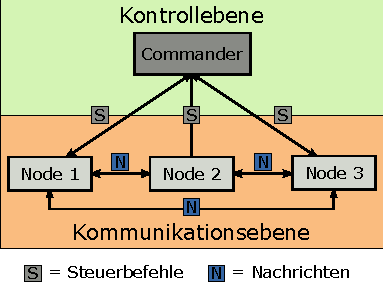
\includegraphics[width=8cm]{CodeAufbau.pdf}
	\caption[Aufbau der Anwendung]{Schematischer Aufbau des implementierten verteilten Systems. Jeder Node ist ein eigenständiger Prozess welcher jeweils auf einer eigenen virtuellen Maschine läuft. Der Commander wird auf einer der VMs ausgeführt und koodiniert die Kommunikation zwischen den Nodes. Dadurch wird die Kommunikation eines verteilten Systems simuliert.}
	\label{figure:systemaufbau}
\end{figure}

Die Implementierung wurde in zwei unabhängige Programmteile aufgeteilt. Diese sind ein Commander sowie Nodes. Durch diese Unterteilung ergibt sich entsprechend wie in Abbildung~\ref*{figure:systemaufbau} dargestellt eine logische Aufteilung der Kommunikation im System in eine Kontrollebene sowie eine Kommunikationsebene. Der Commander stellt sozusagen eine übergeordnete Kommandozentrale dar, welche die Kommunikation der Nodes untereinander durch gewisse Steuerbefehle koordiniert. Er besitzt eine grafische Oberfläche, welche mittels WPF erstellt wurde. Für jeden Prozess ist in dem Hauptfenster des Commanders eine eigene Spalte vorhanden, in welcher die aktuellen Informationen des Prozesses angezeigt werden. Abbildung~\ref{figure:commanderWindow} zeigt diese Aufteilung nach Prozessen. Nach dem Start des Commanders wird zudem überprüft, ob die Prozesse im System erreichbar sind. Dies wird durch einen einfachen Ping an die Netzwerkaddresse der Nodes durchgeführt. Der Kommander dient allgemein dazu, die Übersicht über das verteilte System sowie die aktuellen Zustände der Nodes auf den verteilten VMs zu behalten. 

\begin{figure}[ht]
	\centering
	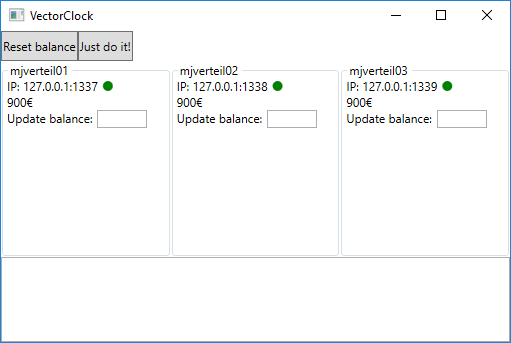
\includegraphics[width=8cm]{commanderWindow.png}
	\caption[Commander Window]{Abbildung des Commanderfensters, welcher dazu dient, die Kommunikation zwischen den Nodes durch Steuerbefehle zu koordinieren}
	\label{figure:commanderWindow}
\end{figure}

Ein Node stellt einen Prozess in dem simulierten System dar. In diesem werden Events ausgeführt und Vektoruhren verarbeitet. Jeder Node besitzt seine eigene, lokale Vektoruhr. Bei einem Node handelt es sich um ein Kommandozeilenprogramm, welches auf einer VM läuft und ständig auf Nachrichten wartet. Damit der Ablauf der Kommunikation besser nachvollzogen werden kann, gibt ein Node bei jedem Event die Details der Nachricht sowie seiner Vektoruhr aus. Eine Darstellung des Node Fensters zeigt Abbildung~\ref{figure:nodeWindow}. Zusätzlich zu der eigenen Ausgabe sendet er dabei eine Antwort an den Commander mit der Nachricht, welche er erhalten hat sowie seiner aktuellen lokalen Uhr. Der Commander gibt diese empfangene Antwort in einem Textfenster aus und aktualisiert zudem die einzelnen Statusanzeigen im Mainwindow. Eine Beispielhafte Darstellung solch einer empfangenen Nachricht mit darauf folgender Ausgabe des Inhalts ist in Abbildung  dargestellt.

\begin{figure}[ht]
	\centering
	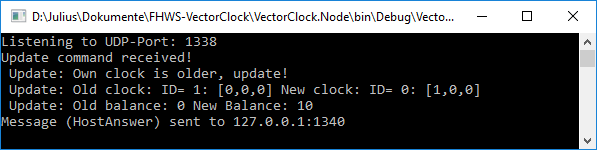
\includegraphics[width=10cm]{nodeWindow.png}
	\caption[Node Window]{Abbildung des Nodefensters. Zwischen den Nodes findet die eigentlichen Kommunikation statt.}
\label{figure:nodeWindow}
\end{figure}

Die Kommunikation zwischen dem Commander und den Nodes wurde mittels UDP realisiert. Die Entscheidung viel auf UDP, da sich dadurch unnötiger Overhead und Programmieraufwand vermeiden lässt, welcher beispielsweise bei TCP angefallen wäre. Der Unterschied liegt hierbei in Art der Verbindung. UPD ist ein Verbindungsloses Protokoll, bei dem Nachrichten nur an einen Empfänger verschickt werden und dieser nicht darauf antwortet. Bei TCP hingegen muss vor der eigentlichen Kommunikation ein Verbindungsaufbau stattfinden, was zwangsweise in erhöhtem Overhead resultiert \cite*{Markert2013}.

Wichtig für die Beschreibung der Architektur ist auch der Aufbau der ausgetauschten Nachrichten. Dieser ist in Abbildung~\ref{figure:aufbauNachricht} dargestellt. Generell lässt sich ein Nachrichtenobjekt in drei Bestandteile aufteilen. Diese sind ein Header, ein Control- sowie Communicationblock. 

\begin{figure}[ht]
	\centering
	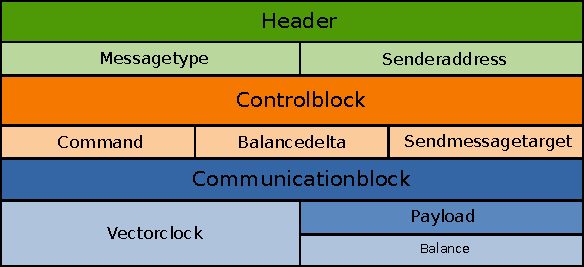
\includegraphics[width=10cm]{AufbauNachricht.pdf}
	\caption[Aufbau einer Nachricht]{Aufbau einer Nachricht zwischen Commander und den Nodes. Diese besteht aus einem Header zur Addressierung, einem Controlblock für die Kommunikation mit dem Commander sowie einem Communicationblock zur Kommunikation der Nodes untereinander.}
	\label{figure:aufbauNachricht}
\end{figure}

Im Header stehen Messagetype sowie Senderaddress. Diese werden dafür verwendet, die Nachricht zu adressieren und bei Empfang die Art der Verarbeitung festzulegen. Dies kann zum Einen Steuerung oder zum anderen Kommunikation sein.

Der Controlblock beinhaltet den Command, das Balancedelta und das Sendmessagetarget. Durch den Command kann der Commander einen Steuerbefehl direkt an einzelne Nodes übersenden und diesem so mitteilen, was er zu tun hat. Sollte eine Kontoaktualisierung gewünscht sein, wird der zu ändernde Betrag in Balancedelta eingetragen. Falls ein Node eine Nachricht an einen anderen senden soll, befindet sich die Adresse des Empfängers in der Variable Sendmessagetarget.

Im Falle einer Kommunikationsnachricht kommt der Communicationblock zum tragen. Der wichtigste Bestandteil ist hierbei die Vektoruhr, denn bei jeder Kommunikationsnachricht muss die aktuelle Vektoruhr versendet werden. Neben der Uhr beinhaltet dieser Block noch den Payload. Dabei handelt es sich sozusagen um die \qq{Ladung} der Nachricht, welcher im Gegensatz zu der Uhr nur auf der Anwendungsebene interessant ist. In dem hier beschriebenen Bankenbeispiel beinhaltet der Payload die Änderung des Kontostandes durch das aufgetretende Event. Somit werden keine absoluten Werte übertragen, sondern lediglich Änderungsinformationen.

Beim Absenden der Nachricht, egal ob im Commander oder in den Nodes, wird diese serialisiert und per UDP versendet. Im Empfangsfall muss der empfangene Datenstrom wieder deserialisiert und in eine Nachricht umgewandelt werden. Sowohl Serialisierung als auch Deserialisierung wir durch die Klasse textit{MessageSerializer} gehandhabt, welche intern auf die Funktionen der Klasse \textit{BinaryFormatter} zugreift.

\FloatBarrier
\subsubsection{Austausch von Nachrichten}
\label{empfangVonNachrichten}
Sowohl der Commander als auch alle Nodes warten ständig während der Ausführung auf ankommende Nachrichten. Dies wurde im Code durch eine While-Schleife implementiert.

\begin{lstlisting}[label=lst:nodeWhile,
language=sharpc,
float=ht,
firstnumber=1,
captionpos=b,
caption=While-Scheife für das Warten auf neue Nachrichten. Auszug aus dem Node.]
using (UdpClient client = new UdpClient(port, AddressFamily.InterNetwork))
{
	while (true)
	{
		IPEndPoint remoteEP = null;
		byte[] data = client.Receive(ref remoteEP);

		Message msg = MessageDeserializer.Deserialize(data);
		controlLogic.HandleMessage(causallyOrderedMode, msg, remoteEP);
	}
}
\end{lstlisting}

Die in Listing~\ref{lst:nodeWhile} dargestellte While-Scheilfe stammt aus dem Node-Teil des Programms. Hier kann die Schleife direkt in der Main-Methode ausgeführt werden, da die einzige Aufgabe des Nodes das Warten auf ankommende Nachrichten ist. Sobald eine Nachricht empfangen wurde, wird die Methode \code{client.Receive()} ausgelöst. Solange keine Nachricht empfangen wird, blockiert die Methode. Anschließend kann die Nachricht aus dem ankommenden Bytestrom deserialisiert und durch den Aufruf \code{controlLogic.HandleMessage()} an die Kontrollebene zur weiteren Verarbeitung übergeben werden. Auf dieser Ebene wird dann entschieden, ob die Nachricht eine Kontroll- oder eine Kommunikationsnachricht ist und anschließend entsprechend gehandelt.

Da es sich bei dem Commander um eine WPF-Anwendung handelt, darf hier die eben beschriebene Schleife das Programm nicht blockieren. Aus diesem Grund wird was Warten auf Antworten der Nodes im Commander in einem Task ausgeführt, welcher dann asynchron auf Antworten wartet.

\begin{lstlisting}[label=lst:commanderWhile,
language=sharpc,
float=ht,
firstnumber=1,
captionpos=b,
caption=Starten eines neuen Tasks um asynchron auf eventuelle Rückantworten der Nodes zu warten.]
public MainViewModel()
{
Node1 = new NodeViewModel("mjverteil01", System.Net.IPAddress.Parse("10.10.29.21"));
Node2 = new NodeViewModel("mjverteil02", System.Net.IPAddress.Parse("10.10.29.142"));
Node3 = new NodeViewModel("mjverteil03", System.Net.IPAddress.Parse("10.10.29.67"));

CheckNodeConnectivities();

Task listenToNodeTask = new Task(async () => await ListenToNode());
listenToNodeTask.Start();
}
\end{lstlisting}

Wie in Listing~\ref{lst:commanderWhile} zu sehen ist, wird am Ende des MainViewModel-Konstruktors nach dem Abfragen des Status für alle Nodes ein neuer Task \code{listenToNodeTask} erzeugt. Dieser bekommt die Methode \code{ListenToNode()} übergeben, in welcher eine ähnliche While-Schleife ausgeführt wird wie in Listing~\ref{lst:nodeWhile}. Am Ende des Konstruktors wird der Task gestartet und das asynchrone Warten auf Nachrichten beginnt.

Das Absenden von Nachrichten funktioniert ähnlich wie das Versenden. Dabei sind die Methoden sowohl im Commander als auch den Nodes die selben, erneut jedoch mit der Einschränkung, dass bei dem Commander wieder die asynchrone Variante der Send-Methode auf dem UdpClient aufgerufen werden muss. 

\begin{lstlisting}[label=lst:sendMessageTo,
language=sharpc,
float=ht,
firstnumber=1,
captionpos=b,
caption=Absenden einer Nachricht in einem Node.]
 private void SendMessageTo(String messageText, Message msg, IPEndPoint node)
 {
	 if(this.endPoint.Equals(node))
		 throw new InvalidOperationException("Sendmessage: Endpoints are equal!");
		 
	 using (UdpClient client = new UdpClient())
	 {
		 client.Connect(node);
		 byte[] data = MessageSerializer.Serialze(msg);
		 client.Send(data, data.Length);
		 Console.WriteLine($"Message ({messageText}) sent to {node}");
	 }
 }
\end{lstlisting}

Der Methode \code{SendMessageTo()} in Listing~\ref{lst:sendMessageTo} wird ein Nachrichtentext, die Nachricht selber sowie ein IPEndPoint übergeben. Der Nachrichtentext dient lediglich der Anzeige auf der Kommandozeile. Die eigentliche Nachricht wird vor dem Absenden durch die Klassen \code{MessageSezializer} zu einem Bytestrom serialisiert und anschließend durch den Client an die in dem IPEndPoint angegebene Zieladdresse verschickt.

Ähnlich wie im Node-Teil des Programms läuft der Sendevorgang wie bereits erwähnt im Commander auch ab. Die Besonderheit ist hier, dass die Nodes als eigenes Objekt des Typs \code{NodeViewModel} gespeichert werden und die Send-Methode direkt auf dem jeweiligen Node ausgeführt wird. Die implizite Angabe einer Zieladdresse fällt hier weg, da diese bereits in den Nodes gespeichert wird.
\subsubsection{Verarbeitung von Nachrichten im Node}
Für die Implementierung der Vektoruhren ist die Behandlung von empfangenen Nachrichten in einem Node besonders interessant. An dieser Stelle kommen die Uhren, Aktualisierungen dieser sowie eventuelle Vergleiche und API-Aufrufe ins Spiel. 

\begin{lstlisting}[label=lst:handleMessageIncrease,
language=sharpc,
float=ht,
firstnumber=1,
captionpos=b,
caption=Auszug aus der \code{HandleControlMessage()}-Methode. Hier wird ein UpdateBalance-Befehl verarbeitet.]
 else if (msg.controlBlock.Command == ControlCommand.UpdateBalance)
 {
	 Console.WriteLine("Increase command received!");
	 commLogic.appLogic.UpdateBalance(msg.controlBlock.BalanceDelta);
	 Console.WriteLine($"New balance: {commLogic.appLogic.balance}");
	 commLogic.IncreaseVectorClock();                                    
	 Console.WriteLine($"New Clock: {this.commLogic.clock}");
	 BroadcastChange(msg);
	 returnValue = true;
 }
\end{lstlisting}

In dem Programmablauf findet eine Verarbeitung nach dem Empfang statt, welcher in Abschnitt~\ref{empfangVonNachrichten} bereits behandelt wurde. Wie beschrieben findet anhand des Befehls, welcher in dem Kontroll-Block der Nachricht enthalten ist, eine Verzweigung in Kontroll-Ebene und Kommuni"-kations-Ebene statt. Nach dieser Verzweigung wird in der selben Methode immer eine Antwortnachricht an den Commander erstellt und abgeschickt, welche die aktuelle lokale Vektoruhr sowie den Payload der Applikationslogik enthält.

Liegt eine Nachricht auf Kontrollebene vor, welche demnach von dem Commander stammt, wird die darin enthaltenen Aktion ausgeführt. Dies kann entweder eine Kontostandaktualisierung mit anschließendem Broadcast, die Aufforderung zum Senden einer Nachricht an einen anderen einzelnen Node oder ein allgemeiner Befehl wie beispielsweise \code{Shutdown} sein. Ein Auszug aus der Implementierung ist in Listing~\ref{lst:handleMessageIncrease} abgebildet.

Im Fall einer Kommunikationsnachricht wird diese entsprechend der in Abschnitt~\ref{prinzipFunktion} erläuterten Funktionsweise behandelt. Dies beinhaltet das Aktualisieren der lokalen Vektoruhr anhand der Uhr, welche an die Nachricht angehängt ist. Zudem wird der Payload verarbeitet, also in dem Kontext des Banken-Szenarios der Kontostand aktualisiert. Diese Aktualisierung ist hierbei bereits Aufgabe der Anwendungsschicht und kann somit gleichgesetzt werden mit einem API-Aufruf. Die Zusammenhänge dieser Thematik werden in Abschnitt~\ref{RolleDerAnwendung} genauer betrachtet.


